\section{Visualizing Profiler Outputs}

Several useful plotting methods have been provided in the \pkg{pbdPROF} package for visualizing fpmpi and mpiP profiler outputs.  

In addition, the data is stored in a fairly simple format, so it should be simple enough to create your own plots if these do not suffice.

\subsection{Visualizing fpmpi Profiler Output}

\begin{figure}
  \centering
  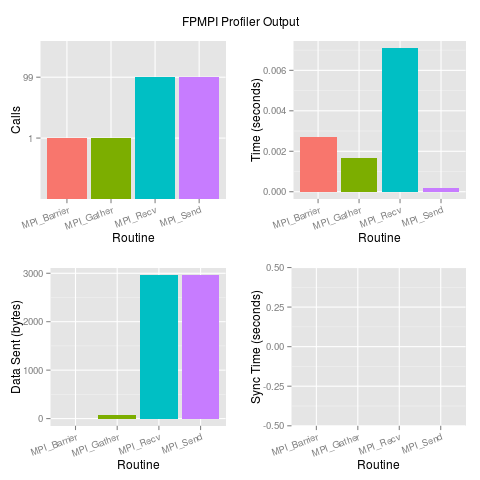
\includegraphics[width=0.485\textwidth]{include/pics/fpmpi}
  \caption{fpmpi Plots}
  \label{fig:fpmpi}
\end{figure}


\subsection{Visualizing mpiP Profiler Output}

\begin{figure}
        \centering
        \begin{subfigure}[b]{0.485\textwidth}
            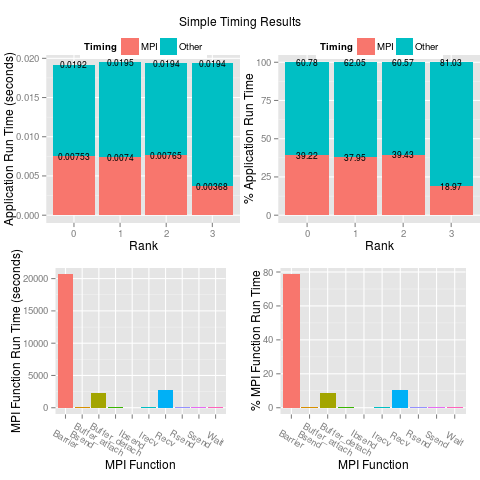
\includegraphics[width=\textwidth]{include/pics/mpip/01_timing}
        \end{subfigure}%
        \hspace{.2cm}
        \begin{subfigure}[b]{0.485\textwidth}
            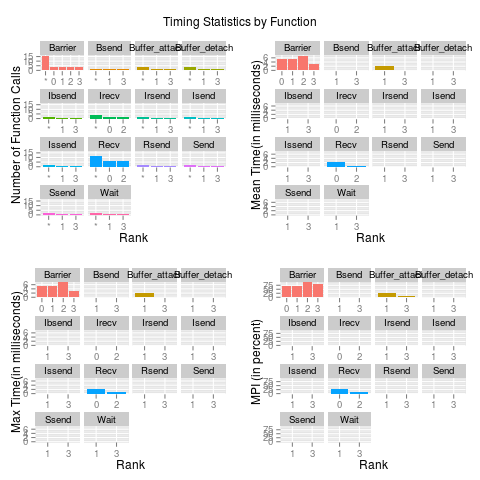
\includegraphics[width=\textwidth]{include/pics/mpip/02_stats}
        \end{subfigure}\\
        \begin{subfigure}[b]{0.485\textwidth}
            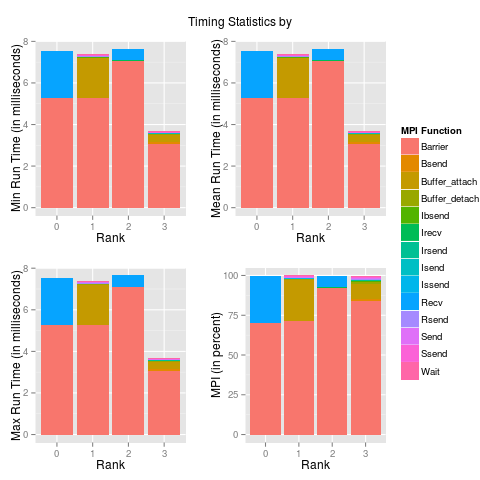
\includegraphics[width=\textwidth]{include/pics/mpip/03_other}
        \end{subfigure}%
        \hspace{.2cm}
        \begin{subfigure}[b]{0.485\textwidth}
            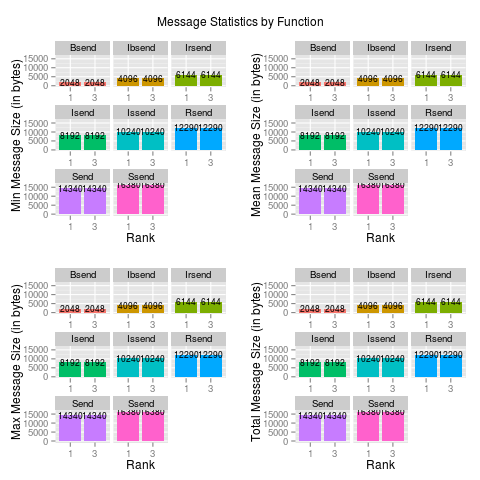
\includegraphics[width=\textwidth]{include/pics/mpip/04_message}
        \end{subfigure}\\
        \begin{subfigure}[b]{0.485\textwidth}
            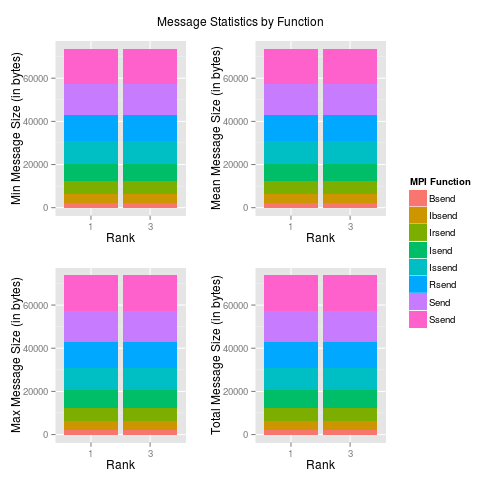
\includegraphics[width=\textwidth]{include/pics/mpip/05_message2}
        \end{subfigure}%
        \caption{mpiP Plots}
        \label{fig:mpip}
\end{figure}